%% BioMed_Central_Tex_Template_v1.06
%%                                      %
%  bmc_article.tex            ver: 1.06 %
%                                       %

%%IMPORTANT: do not delete the first line of this template
%%It must be present to enable the BMC Submission system to
%%recognise this template!!

%%%%%%%%%%%%%%%%%%%%%%%%%%%%%%%%%%%%%%%%%
%%                                     %%
%%  LaTeX template for BioMed Central  %%
%%     journal article submissions     %%
%%                                     %%
%%          <8 June 2012>              %%
%%                                     %%
%%                                     %%
%%%%%%%%%%%%%%%%%%%%%%%%%%%%%%%%%%%%%%%%%


%%%%%%%%%%%%%%%%%%%%%%%%%%%%%%%%%%%%%%%%%%%%%%%%%%%%%%%%%%%%%%%%%%%%%
%%                                                                 %%
%% For instructions on how to fill out this Tex template           %%
%% document please refer to Readme.html and the instructions for   %%
%% authors page on the biomed central website                      %%
%% http://www.biomedcentral.com/info/authors/                      %%
%%                                                                 %%
%% Please do not use \input{...} to include other tex files.       %%
%% Submit your LaTeX manuscript as one .tex document.              %%
%%                                                                 %%
%% All additional figures and files should be attached             %%
%% separately and not embedded in the \TeX\ document itself.       %%
%%                                                                 %%
%% BioMed Central currently use the MikTex distribution of         %%
%% TeX for Windows) of TeX and LaTeX.  This is available from      %%
%% http://www.miktex.org                                           %%
%%                                                                 %%
%%%%%%%%%%%%%%%%%%%%%%%%%%%%%%%%%%%%%%%%%%%%%%%%%%%%%%%%%%%%%%%%%%%%%

%%% additional documentclass options:
%  [doublespacing]
%  [linenumbers]   - put the line numbers on margins

%%% loading packages, author definitions

%\documentclass[twocolumn]{bmcart}% uncomment this for twocolumn layout and comment line below
\documentclass{bmcart}

%%% Load packages
%\usepackage{amsthm,amsmath}
%\RequirePackage{natbib}
%\RequirePackage{hyperref}
\usepackage[utf8]{inputenc} %unicode support
%\usepackage[applemac]{inputenc} %applemac support if unicode package fails
%\usepackage[latin1]{inputenc} %UNIX support if unicode package fails
\usepackage{graphicx,subfigure}

%%%%%%%%%%%%%%%%%%%%%%%%%%%%%%%%%%%%%%%%%%%%%%%%%
%%                                             %%
%%  If you wish to display your graphics for   %%
%%  your own use using includegraphic or       %%
%%  includegraphics, then comment out the      %%
%%  following two lines of code.               %%
%%  NB: These line *must* be included when     %%
%%  submitting to BMC.                         %%
%%  All figure files must be submitted as      %%
%%  separate graphics through the BMC          %%
%%  submission process, not included in the    %%
%%  submitted article.                         %%
%%                                             %%
%%%%%%%%%%%%%%%%%%%%%%%%%%%%%%%%%%%%%%%%%%%%%%%%%


%\includegraphic{}
%\includegraphics{}



%%% Put your definitions there:
\startlocaldefs
\endlocaldefs


%%% Begin ...
\begin{document}

%%% Start of article front matter
\begin{frontmatter}

\begin{fmbox}
\dochead{Research}

%%%%%%%%%%%%%%%%%%%%%%%%%%%%%%%%%%%%%%%%%%%%%%
%%                                          %%
%% Enter the title of your article here     %%
%%                                          %%
%%%%%%%%%%%%%%%%%%%%%%%%%%%%%%%%%%%%%%%%%%%%%%

\title{Methods to compute the composite log-likelihood (CLL) of allelic
  frequencies for the detection of
  signatures of selection in diploid genomes}

%%%%%%%%%%%%%%%%%%%%%%%%%%%%%%%%%%%%%%%%%%%%%%
%%                                          %%
%% Enter the authors here                   %%
%%                                          %%
%% Specify information, if available,       %%
%% in the form:                             %%
%%   <key>={<id1>,<id2>}                    %%
%%   <key>=                                 %%
%% Comment or delete the keys which are     %%
%% not used. Repeat \author command as much %%
%% as required.                             %%
%%                                          %%
%%%%%%%%%%%%%%%%%%%%%%%%%%%%%%%%%%%%%%%%%%%%%%

\author[
   addressref={aff1},                   % id's of addresses, e.g. {aff1,aff2}
   corref={aff1},                       % id of corresponding address, if any
   %noteref={n1},                        % id's of article notes, if any
   email={filippo.biscarini@tecnoparco.org}   % email address
]{\inits{FB}\fnm{Filippo} \snm{Biscarini}}
\author[
   addressref={aff1}, 
   email={nelson.nazzicari@tecnoparco.org}
]{\inits{NN}\fnm{Nelson} \snm{Nazzicari}}
\author[
   addressref={aff1}, 
   email={john.RS.Smith@cambridge.co.uk}
]{\inits{AS}\fnm{Alessandra} \snm{Stella}}

%%%%%%%%%%%%%%%%%%%%%%%%%%%%%%%%%%%%%%%%%%%%%%
%%                                          %%
%% Enter the authors' addresses here        %%
%%                                          %%
%% Repeat \address commands as much as      %%
%% required.                                %%
%%                                          %%
%%%%%%%%%%%%%%%%%%%%%%%%%%%%%%%%%%%%%%%%%%%%%%

\address[id=aff1]{%                           % unique id
  \orgname{Department of Bioinformatics, PTP}, % university, etc
  \street{Via Einstein - Loc. Cascina Codazza},                     %
  %\postcode{26900}                                % post or zip code
  \city{Lodi},                              % city
  \cny{Italy}                                    % country
}
%\address[id=aff2]{%
%  \orgname{Marine Ecology Department, Institute of Marine Sciences Kiel},
%  \street{D\"{u}sternbrooker Weg 20},
%  \postcode{24105}
%  \city{Kiel},
%  \cny{Germany}
%}

%%%%%%%%%%%%%%%%%%%%%%%%%%%%%%%%%%%%%%%%%%%%%%
%%                                          %%
%% Enter short notes here                   %%
%%                                          %%
%% Short notes will be after addresses      %%
%% on first page.                           %%
%%                                          %%
%%%%%%%%%%%%%%%%%%%%%%%%%%%%%%%%%%%%%%%%%%%%%%

\begin{artnotes}
%\note{Sample of title note}     % note to the article
%\note[id=n1]{Equal contributor} % note, connected to author
\end{artnotes}

\end{fmbox}% comment this for two column layout

%%%%%%%%%%%%%%%%%%%%%%%%%%%%%%%%%%%%%%%%%%%%%%
%%                                          %%
%% The Abstract begins here                 %%
%%                                          %%
%% Please refer to the Instructions for     %%
%% authors on http://www.biomedcentral.com  %%
%% and include the section headings         %%
%% accordingly for your article type.       %%
%%                                          %%
%%%%%%%%%%%%%%%%%%%%%%%%%%%%%%%%%%%%%%%%%%%%%%

\begin{abstractbox}

\begin{abstract} % abstract
\parttitle{First part title} %if any
Text for this section.

\parttitle{Second part title} %if any
Text for this section.
\end{abstract}

%%%%%%%%%%%%%%%%%%%%%%%%%%%%%%%%%%%%%%%%%%%%%%
%%                                          %%
%% The keywords begin here                  %%
%%                                          %%
%% Put each keyword in separate \kwd{}.     %%
%%                                          %%
%%%%%%%%%%%%%%%%%%%%%%%%%%%%%%%%%%%%%%%%%%%%%%

\begin{keyword}
\kwd{composite log-likelihood}
\kwd{signatures of selection}
\kwd{diploid genomes}
\end{keyword}

% MSC classifications codes, if any
%\begin{keyword}[class=AMS]
%\kwd[Primary ]{}
%\kwd{}
%\kwd[; secondary ]{}
%\end{keyword}

\end{abstractbox}
%
%\end{fmbox}% uncomment this for twcolumn layout

\end{frontmatter}

%%%%%%%%%%%%%%%%%%%%%%%%%%%%%%%%%%%%%%%%%%%%%%
%%                                          %%
%% The Main Body begins here                %%
%%                                          %%
%% Please refer to the instructions for     %%
%% authors on:                              %%
%% http://www.biomedcentral.com/info/authors%%
%% and include the section headings         %%
%% accordingly for your article type.       %%
%%                                          %%
%% See the Results and Discussion section   %%
%% for details on how to create sub-sections%%
%%                                          %%
%% use \cite{...} to cite references        %%
%%  \cite{koon} and                         %%
%%  \cite{oreg,khar,zvai,xjon,schn,pond}    %%
%%  \nocite{smith,marg,hunn,advi,koha,mouse}%%
%%                                          %%
%%%%%%%%%%%%%%%%%%%%%%%%%%%%%%%%%%%%%%%%%%%%%%

%%%%%%%%%%%%%%%%%%%%%%%%% start of article main body
% <put your article body there>

%%%%%%%%%%%%%%%%
%% Background %%
%%%%%%%%%%%%%%%%
\section*{Background}
Selection, both natural and artificial, is one of the major forces that
can shape the genome of living organisms and change allele frequencies.
A mutation that is beneficial for the adaptation of an organism to its
environment, or that is of agricultural or industrial interest, tends to increase in
frequency in the population, together with neighbouring genomic regions
which are dragged along (``hitch-hiked'') in the process (\cite{braverman1995hitchhiking}). 
Through the last decade, the on-going genomic revolution has been making
available hundreds of thousands of genetic markers for several animal, microbial and
plant species. By looking at the allele frequency at marker loci along
the genome of populations experiencing different selective pressures, it
is possible to identify genomic regions -and ultimately genes- involved
in processes such as domestication, adaptation, evolution and artificial
selection. There are a number of methods based on allele frequencies
that have been developed to detect such signatures of selection. A
popular method is Wright's $F_{ST}$
(\cite{wright1949genetical,nei1977f}) that has been applied to
studies in humans (\cite{akey2002interrogating}), plants
(\cite{zhao2010genomic}) and animals (\cite{kijas2012genome}).
Alternatively, the likelihood of the difference between allele
frequencies in different populations can be estimated and used to detect
the presence of signatures of selection
(\cite{nielsen2005genomic,stella2010identification}).
However, there are several ways in which such likelihoods can be
computed, and these might differ in computation requirements and
statistical properties, such as the sensitivity to detect signals of
selection or the behaviour along the margins of the dimensional space.
It may therefore be of interest to investigate the statistical
properties of different estimators
for the likelihood of the difference between allele frequency, and
assess how well they are capable of detecting actual signals of
selection.

In this study we evaluated 4 different ways to estimate the likelihood
of the difference in allele frequency between populations. The logarithm
of the likelihoods thus calculated were then computed and combined across sliding windows
along the genome (CLL, composite log-likelihood) in order to detect
signatures of selection. The proposed CLL approaches were compared among
them and with approaches based on $F_{ST}$ and on simple squared
distances between genotypes. All methods were first analysed numerically
 by simulating scenarios along the entire dimensional space (frequency range
 and population size ratios between the test and null populations) and then tested with real data where strong signals
of selection are known to be present. The methods hereby presented have
been developed having in mind biallelic genetic markers (namely SNPs),
but can in principle be adapted to any kind of markers and applied to
any diploid organism.

\section*{Methods}

Let's assume we have a test population \emph{T} (the population on which we want to detect
signatures of selection) and a null or reference population \emph{N} (the
contrasting population(s)). On these populations $F_{ST}$, the squared
difference of the allelic frequencies, and four different likelihood
measures of allele frequency differences have been computed and
evaluated in terms of their ability to detect signatures of selection. 
First, we present numerical details of the different calculations, then
examples with real data on which the different estimators were tested.


\subsection*{Detecting signatures of selection}
\subsubsection*{$F_{ST}$}
The $F_{ST}$ (Wright's \emph{F} statistics for \emph{Subpopulation} vs
\emph{Total}), a.k.a. \emph{fixation index}, is a measure of the genetic
differentiation between (sub)populations (e.g. the test and reference
populations in our case). For any given locus, $F_{ST}$ was calculated as
described by Nei (\cite{nei1977f}); partitioning the total
expected heterozygosity ($H_T$, or gene diversity) into the
\emph{interpopulation} diversity ($D_{ST}$) and the
\emph{intrapopulation} diversity ($\overline{H}_S$),
the $F_{ST}$ is defined as the proportion of gene diversity due to
differentiation among subpopulations:

\begin{equation} \label{eq:fstnei}
F_{st}=\frac{D_{st}}{H_T}=\frac{H_T-\overline{H}_S}{H_T}=1-\frac{\overline{H}_S}{H_T}  
\end{equation}

where $\overline{H}_S=\sum_{i=1}^k w_iH_{S_i}$ is the weighted average of the expected heterozygosities within
\emph{k} subpopulations each accounting for a proportion $w_i$ of the total
population size ($H_{S_i}=1-\sum_{j=1}^{m} p_j^2$
is the expected heterozygosity within subpopulation \emph{i} -with $m$
alleles at the given locus); $H_T=1-\sum_{i=1}^m \overline{p}_{i}^2$
is the expected heterozygosity in the overall
population, with $\overline{p_i}=\sum_{i=1}^k w_k p_k$, the average
allele frequency at the given locus across \emph{k} subpopulations
each accounting for a proportion $w_i$ of the total sample size.

$F_{ST}$ measures the differentiation between the null and reference
populations, and was used in this study as primary benchmark against
which other methods were evaluated. 

\subsubsection*{Squared difference ($D^2$)}
A very simple and naive approach for the estimation of the genetic
distance between populations is the squared difference of their allele
frequencies. For any given locus, the allele frequencies of the first
allele in the test and
null populations ($p_1$ and $p_2$) were calculated, and their squared difference used to
measure the degree of differentiation between the two populations:

\begin{equation}
D^2=(p_1-p_2)^2
\end{equation}

While $F_{ST}$ was chosen as benchamrk due to its long-standing theoretical
development and its wide-spread use in the detection of population
substructure, $D^2$ has been used as additional naive benchmark against which
more sophisticated methods can be compared. 

\subsubsection*{Binomial log-likelihood (BLL)}
Allele frequencies at a given locus (\emph{A/a}) between the test
and null populations are compared. Let $p_N$ be the frequency of
allele \emph{A} in the null population, and $n_T$ and $k_T$ the total number of
alleles and the number of \emph{A} alleles in the test population
respectively. Under the null hypothesis that $p_T=p_N$, the allele count
in the test population can be thought of as a random sample from the
same reference population. The following binomial function measures the likelihood
that such a sample actually comes from the reference population:  

\begin{equation}
BLL_{ij}=ln\left\{{n_T \choose k_T} (1-p_N)^{k_T}p_N^{n_T-k_T}\right\}
\end{equation}

where $BLL_{ij}$ is the probability to observe the test allele
distribution at locus \emph{j} on chromosome \emph{i} in the null population. 
The smaller $BLL_{ij}$ the less likely it is that the two populations are
one and the same, and the more justifiable it is to accept the
alternative hypothesis that the test and null populations are actually
different (for instance because of some genetic processs such as natural or
artificial selection). 

Unless the test and null populations have the same size and their allele
frequencies are complementary ($p_N=p_T$), the binomial log-likelihood
is not symmetric. Therefore, three cases can be envisaged: 1) comparison
of N vs T (\emph{BLL1}); 2) comparison of T vs N (\emph{BLL2}); 3)
  comparison of  T vs N+T (\emph{BLL3}). The latter is what was
  implemented in \cite{stella2010identification}, and works well with
  multiple comparisons, when one population has to be compared against
  many other populations: it has the advantage
  of creating fewer numerical problems (lack of symmetry, falling
  outside of the computational space etc ...), but has the shortcoming
  of shrinking the power of the comparison (since $T \subset N$ -the test population is
  included in the null population). Additionally, it is often the case
  that two populations have to be compared against each other. For the
  reasons above, all three scenarios (\emph{BLL1, BLL2, BLL3}) were
  evaluated in the present study.

\subsubsection*{Multiplicative log-likelihood (MLL)}
To overcome the issue of the lack of symmetry with BLL, a
possibility is to combine the likelihood of BLL1 and BLL2 (T vs N
and N vs T). A natural approach to combining probabilities is through
multiplication. Therefore the multiplicative log-likelihood was defined
as the geometric mean of the two binomial log-likelihoods:

\begin{equation}
MLL_{ij} = \sqrt{BLL_{ij(TvsN)}*BLL_{ij(NvsT)}}
\end{equation}

where $MLL_{ij}$ is the multiplicative log-likelihood at locus \emph{j}
on chromosome \emph{i} and $BLL_{ij(TvsN)}$ and $BLL_{ij(NvsT)}$ are the
two binomial log-likelihoods (BLL1 and BLL2).

\subsubsection*{Hypergeometric log-likelihood (HGLL)}
An alternative approach is to look at the test population as a random
sample from the reference population and calculate the probability of
obtaining the observed allele counts. Under the null hypothesis that $p_N=p_T$, the two populations
can be combined into one and such probability would follow a hypergeometric distribution:

\begin{equation}
HGLL_{ij}=\frac{{n_{A_N}+n_{A_T} \choose n_{A_T}} \cdot {(N_N+N_T)-(n_{A_N}+n_{A_T}) \choose N_T-n_{A_T}}}{{N_N+N_T \choose N_T}}
\end{equation}

where $n_{A_N}$, $n_{A_T}$, $N_N$ and $N_T$ are the number of A alleles
and the total number of
alleles in the null and test population respectively.
HGLL is symmetric with respect to the population chosen as test or
reference (\cite{jantosciak2002duality}), and assumes that sampling is without replacement, which may
be closer to the allele sampling process involved in the biological
differentiation of populations.
 

\subsubsection*{Distribution of the differences (DIFF)}
Instead of comparing the allele frequency observed in the test
population against that of the null population, one could look
directly at the difference between the two allele frequencies. 
First, the absolute difference between allele frequencies is
calculated: $d=|p_1-p_2|$. In order to obtain a likelihood value for
\emph{d}, both an analytical (\emph{DIFF1}) and numerical (\emph{DIFF2})
approach were adopted.
In \emph{DIFF1}, \emph{d} was standardized ($z=\frac{d}{\sqrt{\hat{p}(1-\hat{p})(1/N_N+1/N_T)}}$) and compared against a normal
distribution.
In \emph{DIFF2}, genotypes were randomly permuted between the null and
test population, and the difference between the allele frequencies
calculated each time. A distribution of values of \emph{d} under
\emph{$H_0$} ($d=0$) was thus
produced and its empirical probability distribution function used to obtain a
likelihood value for the allele frequency difference between the
original populations, \emph{d}. Different numbers
of permutations were tested in terms of results obtained and computation
time.

\subsection*{Simulated scenarios}
For all methods for the detection of signatures of selection, different
scenarios were simulated, in order to evaluate the statistical behaviour
and computational requirements for chainging values of the parameters
used. Specifically, the methods were evaluated against different values
of allele frequency and different sample sizes in the null and test
populations. The whole range of allele frequency (from 0 to 1) was
simulated, and three different population size ratios were considered:
balanced design (equally sized null and test population), mildly
unbalanced design (1:2 population size ratio), and extremely unbalanced
design (1:10 population size ratio).

\subsection*{``Ballons d'essai''}

Data from a population of xxx Holstein-Frisian (zzz males and xxx
females) and yyy Piedmontese (males and females?)
cattle were available. The first breed has been long selected for dairy
production, the latter for meat production. All animals were genotyped
with the Bovine 54k SNP-chip. Genotypes were edited for individual and
marker call-rate ($>95\%$ ?) and for MAF ($>0.05$ ?). Remaining missing
genotypes were imputed using (check this!). Xxx SNPs were eventually
available for analysis. We selected the zzz SNPs on chromosome 3 (BTA-3) as
working example to test the different estimators of the CLL of the
allele frequency difference between populations and the reference
methods ($F_{ST}$ and Euclidean distances) for the detection of
signatures of selection.
BTA-3 is known to host, within the gene \emph{SLC35A3} (position:
43400328-43445390 bps, approximately halfay along the chromosome), the point mutation responsible for CVM (Complex
Vertebral Malformation) in Holstein-Frisian cattle (\cite{thomsen2006missense}).  
CVM is a recessive inherited disorder that frequently causes abortion or perinatal
death in Holstein-Frisian calves. Other cattle breeds -including Piedmontese- are not affected by
the condition. A strong signal is therefore expected to be found at this
site, making this an ideally suited comparison to test different methods
for the detection of signatures of selection.

?` Also DGAT1, Myostatin, Caseins ?

\subsection*{Sliding windows}
When analysing actual data, $F_{ST}$ and $D^2$ values, and the likelihoods obtained with all the
methods presented, were combined in sliding windows based on the
base-pair distance (bps) between SNPs, in order to reduce the influence of spurious signals.
A fixed sliding window of 200 kbps (check this! Maybe better 500 kb: see
\cite{qanbari2011application}) was used, and composite log-likelihoods (CLL) were thus obtained:

\begin{equation}
CLL_{i\overline{j}}=\frac{1}{w}\sum_{j=1}^{j+w-1}LL_{ij}
\end{equation}

where $CLL_{i\overline{j}}$ is the composite log-likelihood at position \emph{$\overline{j}$}
(midpoint of the sliding window) on chromosome \emph{i}, and $LL_{ij}$
are the log-likelihood values calculated for all the SNPs between SNP
\emph{j} and 200 kbps ahead of it.

\subsection*{Software}
Code in C/C++ (check with Nelson!) was written to implement all of the statistical methods to
detect signatures of selection presented above. The R programming
environment and Octave (\cite{eaton2002gnu}) for statistical analysis were used to prototype some of the
tests and produce graphical visualization of the results.


\section*{Results and discussion}
All methods were evaluated in terms of their statistical properties
(sensitivity to detect signatures of selection, symmetry around
population subdivision, robustness to unbalanced data, behaviour at the
margin of the dimensional space) and computation requirements.

For biallelic loci, $D^2$ is intrinsically symmetric: $(p_1-p_2)^2 =
((1-p_1)-(1-p_2))^2$

BLL1 and BLL2 go to $+\infty$ at the boundaries of the dimensional space
(when the null and test populations are fixed for alternate alleles at
the given locus). This leads to numerical problems and also to
visualization problems when values of different methods are plotted
together for comparison (BLL1 and BLL2 are shrunken towards the bottom
of the plot area). This can also partly explain why BLL1 (or BLL2) and
MLL appear to follow the same pattern: since $MLL=\sqrt{BLL1*BLL2}$,
when one or both of the BLL go to infinity, the MLL is dragged along
with it.

Is Fst obsolete?

Use haplotypes (e.g. EHH)?

\subsection*{Numerical illustration}

Given its behaviour at the boundaries of the dimensional space (no
numerical problems for $p_1$ or $p_2$ equalling either $0$ or $1$), $F_{ST}$
is powerful to detect fixation (same allele or alternate alleles)
(\cite{biswas2006genomic}). Other methods may be more appropriate to
detect ongoing selection, balancing selection, loci or haplotypes at
moderate frequencies.

\subsubsection*{Boundedness}
\emph{BLL1}, \emph{BLL2} and the derived method \emph{MLL} have no upper
bound: they go to $+\infty$ when alternative alleles are fixed in the
test and null populations

\subsubsection*{Computation time (for permutations only)}
[probably this will not be a paragraph bat will go together with the
discussion on permutations]

Cmmputation times for increasing
number of permutations were investigated. The dimensional space of $d=p_1-p_2$ was
explored for permutations going from $1000$ to $50\,000$, with steps of
$1000$, for a population of 50 diploid individuals (25 each in the test
and null population) and 1 locus; at each step, the whole range of frequency comparisons between
the test and null populations was tested. The relationship between n. of
iterations and computation time is clearly linear, as expected for a
first-order problem. From these results, the
computation time required for larger numbers of permutations can be
extrapolated, and the computation time for a single frequency comparison
and a given n. of permutations derived. For instance, on a \emph{2.0GHz
  AMD Opteron}, if we wished to
explore the entire dimensional space with $100\,000$ permutationas at
each step (as
it's been done in the numerical illustrations for the paper), it would
take approximately 9 hours and 20 minutes.
Or, if one wished to make a one-locus comparison between a test and a null
experimental populations (which is usually the case when looking for
signatures of selection) it would take less than 6 minutes with
$200\,000$ permutations and a sample size of 50. Increasing the sample
size would linearly increase the computation time. With 500 individuals
(250 each in the test and null population if balanced, any other
combination thereof otherwise) the empirical analysis of frequency
difference with $100\,000$ permutations would take approximately $\frac{1}{2}$ hour. The same linear relationship
holds for increasing number of loci. With the same 500 individuals and
$100\,000$ permutations, if
the comparison would involve 1000 loci the analysis would take 500 hours
(20 days!). Parallelization could help reduce
the computation time needed (with 4 cores the last example would go down to 5 days).

A different permutation strategy (check with Nelson and describe) might
be more efficient and computation times.

\subsection*{Application to real data}

\subsection*{Testing significance}

When analysing tens or hundreds of thousands of markers the problem of
multiple comparisons is incurred. This is a known statistical problem in general
(\cite{berry2007difficult}), and specifically in the field of genetic
studies (\cite{lander1994genetic,risch1996future}). As the number of
independent tests increases, the probability of obtaining at least one
false positive, under $H_0$, approaches one. This probability is a
function of the number of tests \emph{n} and of the chosen significance
threshold \emph{\(\alpha\)}: \(P(false\_positive)=1-(1-\alpha)^n\). When, for instance,
50000 SNP markers are tested along the genome in search of signatures of
selection, for $\alpha=0.01$, 500 false positive associations are expected on averege, just
by mere chance. 

A classical approach to controlling the number of false positives is to
apply the Bonferroni correction (\cite{hochberg1988sharper}) and
reject $H_0$ when $p-value \leq  \alpha/m$ (i.e. family-wise error rate,
FWER), where $\alpha$ is the chosen
significance threshold and \emph{m} is the number of tests performed. 
The Bonferroni correction aims to make the number of false positives as
close as possible to zero, and is justified when there is an implicit prior
assumption that the probability that all tests are null is not small
(\cite{westfall1997bayesian,wakefield2008reporting}), but tends to be overly conservative in
many practical applications. For example in our case ...
Can the Bonferroni correction be applied to Fst? And $D^2$? The same holds
for FDR.


\begin{itemize}
\item Bonferroni correction: very strict; implicit prior assumption that the
probability that \emph{all} tests are null ($H_0$ is true) is not small. If we believe
that all tests could be null, then aiming to make the number of false
positives zero is justifiable (\cite{wakefield2008reporting})
\item FDR
\item Permutation test
\end{itemize}

\section*{Conclusions}

%%%%%%%%%%%%%%%%%%%%%%%%%%%%%%%%%%%%%%%%%%%%%%
%%                                          %%
%% Backmatter begins here                   %%
%%                                          %%
%%%%%%%%%%%%%%%%%%%%%%%%%%%%%%%%%%%%%%%%%%%%%%

\begin{backmatter}

\section*{Competing interests}
  The authors declare that they have no competing interests.

\section*{Author's contributions}
    Text for this section \ldots

\section*{Acknowledgements}
  Data (Marras ...)? \ldots

The research leading to these results has received funding from the European
Union Seventh Framework Programme (FP7/2007-2013) under grant agreement
n. 276699 (``NEUTRADAPT'')

``NEXTGEN'' (how?)

%%%%%%%%%%%%%%%%%%%%%%%%%%%%%%%%%%%%%%%%%%%%%%%%%%%%%%%%%%%%%
%%                  The Bibliography                       %%
%%                                                         %%
%%  Bmc_mathpys.bst  will be used to                       %%
%%  create a .BBL file for submission.                     %%
%%  After submission of the .TEX file,                     %%
%%  you will be prompted to submit your .BBL file.         %%
%%                                                         %%
%%                                                         %%
%%  Note that the displayed Bibliography will not          %%
%%  necessarily be rendered by Latex exactly as specified  %%
%%  in the online Instructions for Authors.                %%
%%                                                         %%
%%%%%%%%%%%%%%%%%%%%%%%%%%%%%%%%%%%%%%%%%%%%%%%%%%%%%%%%%%%%%

% if your bibliography is in bibtex format, use those commands:
\bibliographystyle{bmc-mathphys} % Style BST file
\bibliography{cll-biblio}      % Bibliography file (usually '*.bib' )

% or include bibliography directly:
% \begin{thebibliography}
% \bibitem{b1}
% \end{thebibliography}

%%%%%%%%%%%%%%%%%%%%%%%%%%%%%%%%%%%
%%                               %%
%% Figures                       %%
%%                               %%
%% NB: this is for captions and  %%
%% Titles. All graphics must be  %%
%% submitted separately and NOT  %%
%% included in the Tex document  %%
%%                               %%
%%%%%%%%%%%%%%%%%%%%%%%%%%%%%%%%%%%

%%
%% Do not use \listoffigures as most will included as separate files

\section*{Figures}
  \begin{figure}[h!]
  \caption{\csentence{Sample figure title.}
      A short description of the figure content
      should go here.}
      \end{figure}

\begin{figure}[h!]
  \caption{\csentence{Sample figure title.}
      Figure legend text.}
    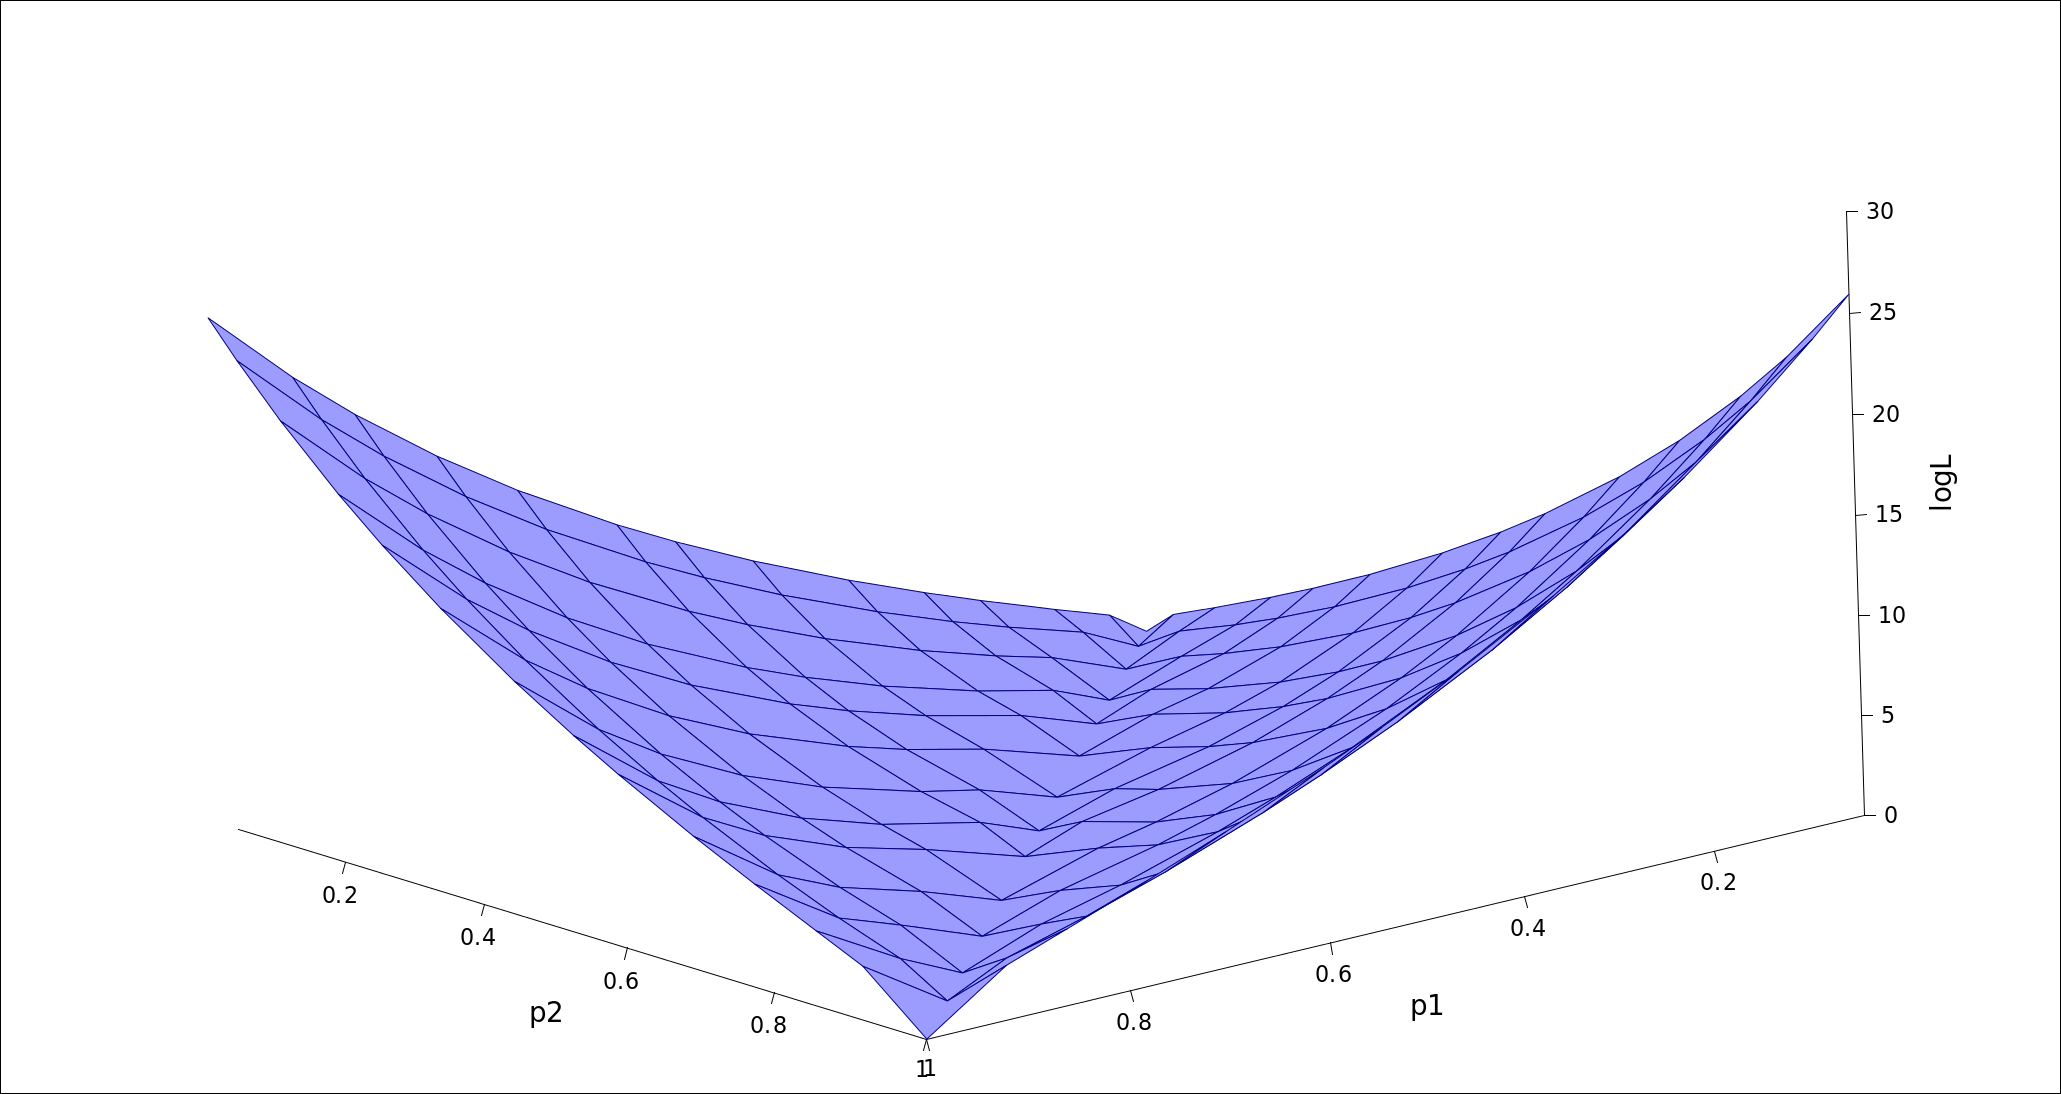
\includegraphics[width=0.9\textwidth]{DiffTest.png}
    \label{fig:difftest}
      \end{figure}

\begin{figure}[ht!]
\begin{center}

% \subfigure[Caption of First Figure]{
%   \label{fig:first}
%   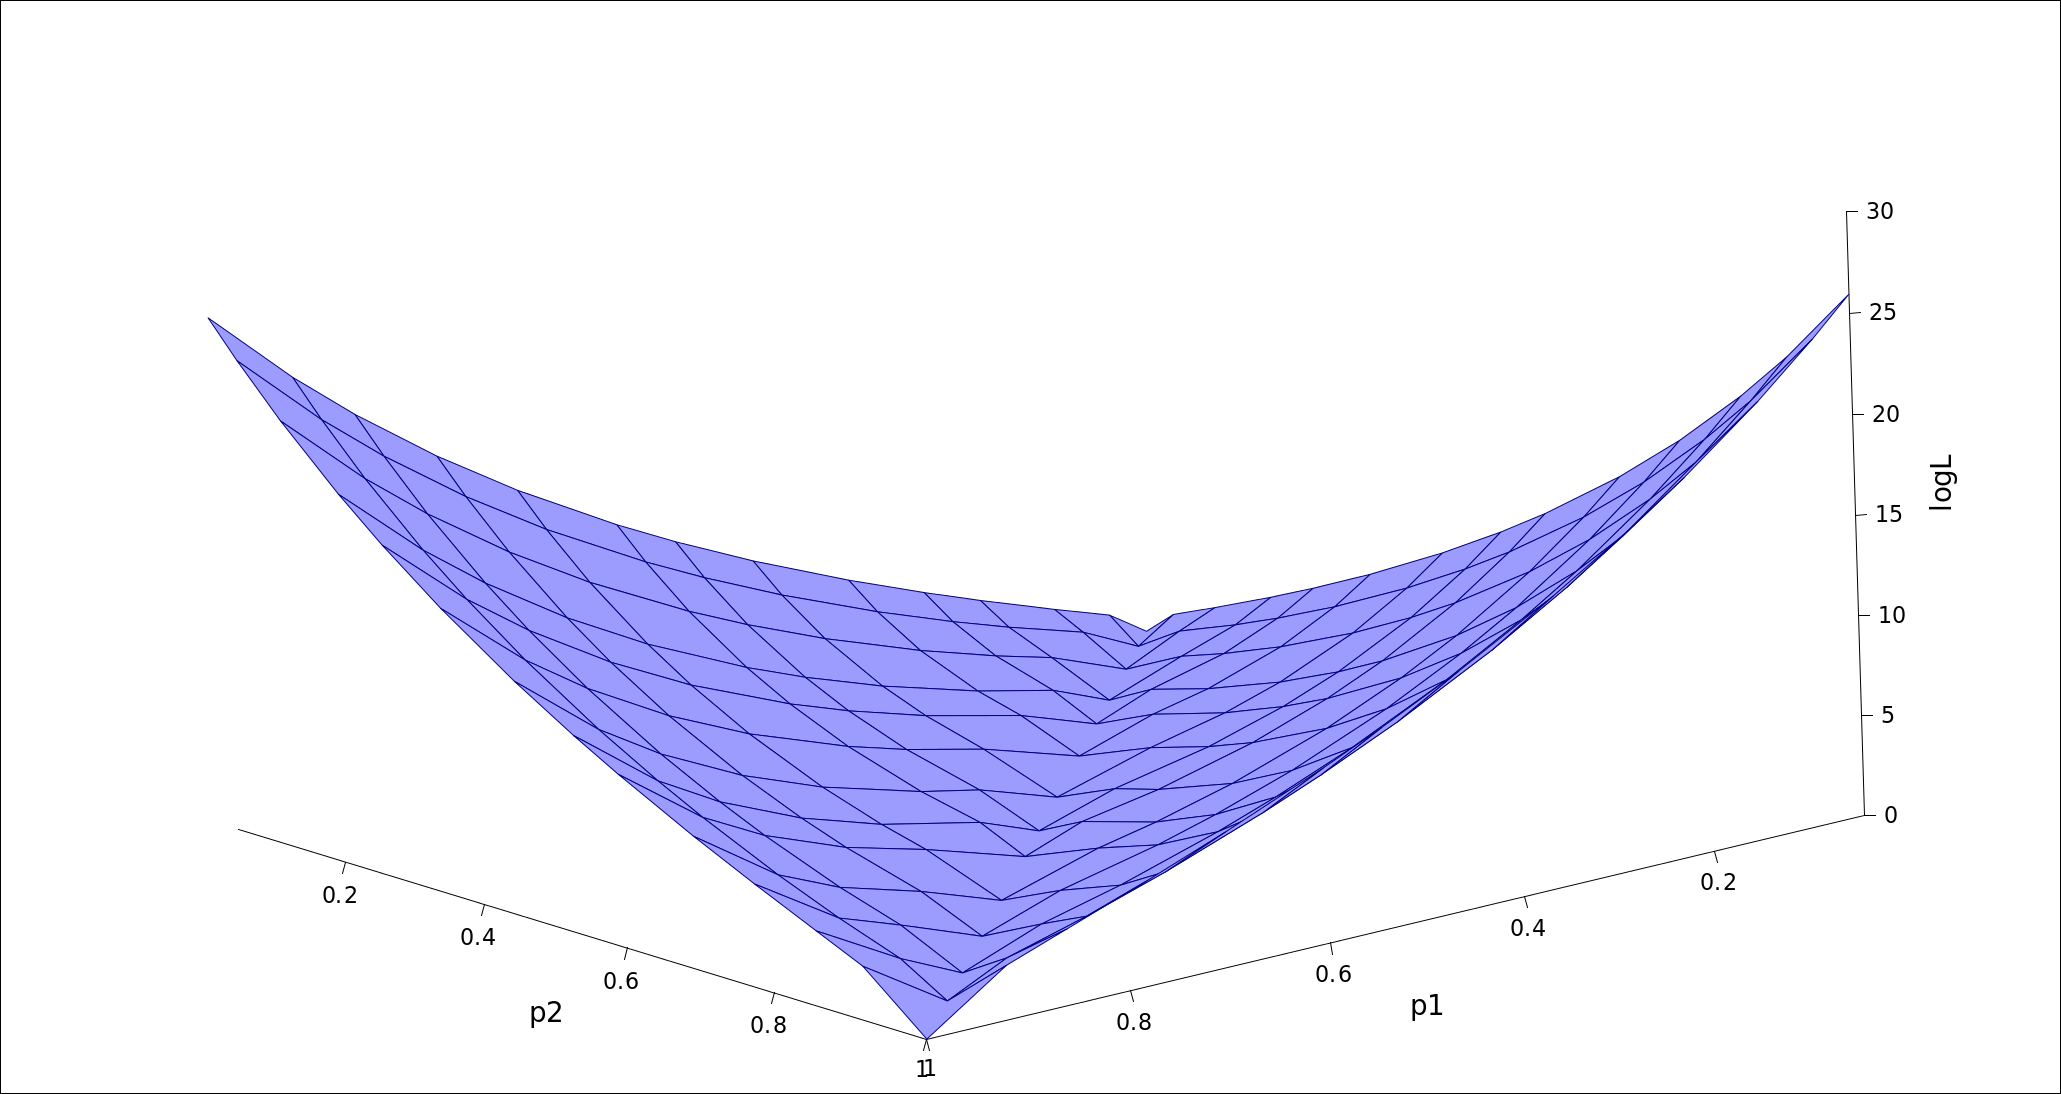
\includegraphics[width=0.4\textwidth]{DiffTest}
% }

% \subfigure[Caption of Second Figure]{
%     \label{fig:second}
%     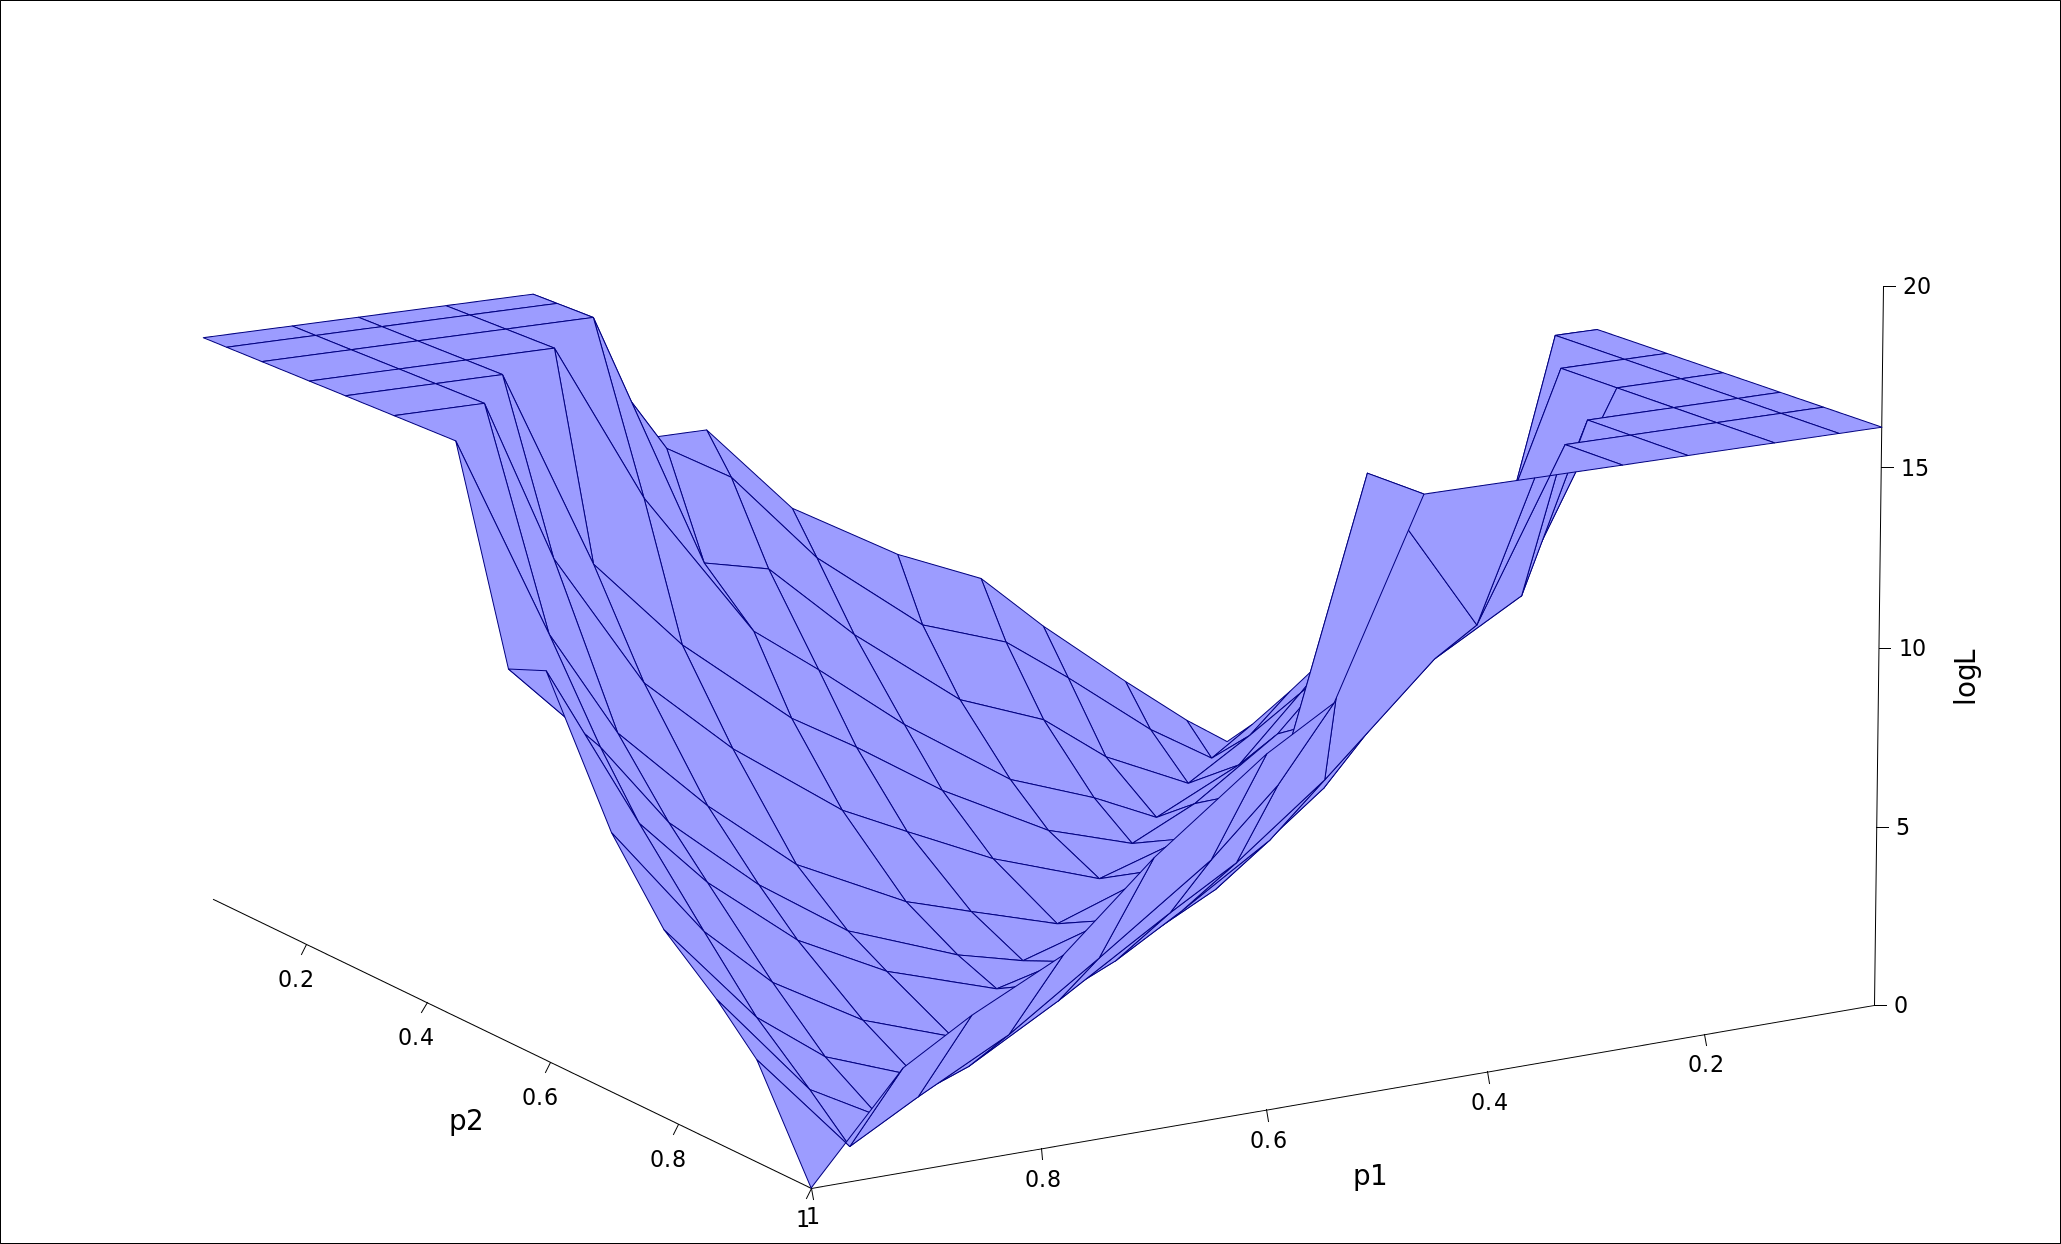
\includegraphics[width=0.4\textwidth]{DiffPermHundredThousand}
%  }\\ % ------- End of the first row ----------------------%

\end{center}
\caption{ 
The l-o-n-g caption for all the subfigures
(FirstFigure through FourthFigure) goes here.
}
\label{fig:subfigures}
\end{figure}

%%%%%%%%%%%%%%%%%%%%%%%%%%%%%%%%%%%
%%                               %%
%% Tables                        %%
%%                               %%
%%%%%%%%%%%%%%%%%%%%%%%%%%%%%%%%%%%

%% Use of \listoftables is discouraged.
%%
\section*{Tables}
\begin{table}[h!]
\caption{Sample table title. This is where the description of the table should go.}
      \begin{tabular}{cccc}
        \hline
           & B1  &B2   & B3\\ \hline
        A1 & 0.1 & 0.2 & 0.3\\
        A2 & ... & ..  & .\\
        A3 & ..  & .   & .\\ \hline
      \end{tabular}
\end{table}

%%%%%%%%%%%%%%%%%%%%%%%%%%%%%%%%%%%
%%                               %%
%% Additional Files              %%
%%                               %%
%%%%%%%%%%%%%%%%%%%%%%%%%%%%%%%%%%%

\section*{Additional Files}
  \subsection*{Additional file 1 --- Sample additional file title}
    Additional file descriptions text (including details of how to
    view the file, if it is in a non-standard format or the file extension).  This might
    refer to a multi-page table or a figure.

  \subsection*{Additional file 2 --- Sample additional file title}
    Additional file descriptions text.


\end{backmatter}
\end{document}
